В контексте трехмерной компьютерной графики, 3D-моделированием (либо трехмерным моделированием) называют процесс разработки
математического представления трехмерной поверхности объектов (живых либо неживых по своей природе) с использованием специальных
инструментов. Продукт трехмерного моделирования -- 3D-модель объекта. Результирующая трехмерная модель может быть отображена
на двухмерном носителе либо напечатана с помощью 3D-принтера либо использована в компьютерной симуляции.

Модели могут быть созданы в автоматическом режеми либо вручную. Процесс ручного создания трехмерной модели по своей сущности
схож с процессом создания скульптуры.

Программное обеспечение трехмерного моделирования, известное под названием 3D-модельер - категория графических приложений, использующихся для создания трехмерных
моделей.

Практически все трехмерные модели могут быть условно поделены на две основные категории.
Цельные -- данные модели определяют объем объекта, который они представляют. Цельные модели в основном используются в инжеренрых и медицинских симуляциях
и обычно строятся с помощью геометрических примитивов.\cite{solid_modelling}

Оболочечные либо поверхностные -- данные модели представляют поверхность объекта (например, сферу шара, либо бесконечно тонкую яичную скорлупу).
Основная область применения таких моделей -- игровая и киноиндустрия, визуализация данных.

Цельные и поверхностные модели функциональ представляют идентичные объекты. Разница между ними в основном состоит в том, каким образом они
определяются и редактируются, а так же набор соглашений используемых при работе с такими моделями, например -- правила и типы аппроксимации
при вычислениях. 

Поверхностные модели должны быть непрерывными (то есть не иметь отверстий, трещин в оболочке) для того чтобы использовать их в
качестве натурального объекта. Полигональные сетки (и, в несколько меньшей степени, подразделенные поверхности) являются наиболее широко распространенной
категорией поверхностных моделей. Горизонтально выровненные наборы полигонов являются полезным инструментов в представлении видоизменяющихся или
деформирующихся поверхностей, подверженных большому числу топологических изменений, таких как, например, поверхность жидкости.

Процесс трансформации представления объектов, например, таких как координаты цетральной точки сферы и ее радиуса, в полигональное представление называется тесселяцией.
Этот процесс генерирует полигональный рендеринг, в котором объекты представленные в виде абстрактных фигур (называемые примитивами - сферы, конусы и т.п) 
преобразуются в полигональные меши, состоящие из сети взаимосвязынных треугольников. 

Меши, существующие в виде треугольников, гораздо популярнее, нежели меши основанные из квадратах, 
потому что было доказано, что они легче поддаются растеризации (поверхность, описываемая каждым треугольником, является плоской, поэтому проекция всегда выпукла).
Полигональное представление не всегда используется в процессе рендеринга, и в этих случаях тесселяция не включена в преобразование из абстрактного представления в конечный результат рендеринга.

% - Процесс моделирования
Существует три популярных пути представления модели:

\begin{enumerate}[label=\arabic*.]
\item Полигональное моделирование (иллюстрация на рисунке \ref{figure:domain:polyface}) -- вершины в трехмерном пространстве, называемые вертексами, соединенные отрезками прямых, формирует полигональную сеть.
Подавляющее большинство существующих трехмерных моделей на сегодня основано на текстурированных полигональных моделях, из-за их гибкости
и возможностей быстрого их отображения.

\begin{figure}[ht]
\centering
  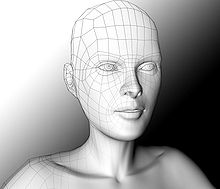
\includegraphics[scale=1.25]{polyface.jpg}
  \caption{Полигональная трехмерная модель человеческого лица}
  \label{figure:domain:polyface}
\end{figure}

\item{Сплайновое моделирование -- метод моделирования, где поверхности определяются с помощью набора кривых,
параметры которых определяются скалярными весами, ассоциированными с контрольными точками. Кривая следует за точками, но не обязательно абсолютно
точно их интерполиует. Увеличение веса точки сдвинет кривую ближе к этой точке.
Наиболее растространенные типы кривых, использующихся при таком методе моделирования:
\begin{itemize}
\item NURBS-кривые;
\item сплайны;
\item сегменты;
\item иные геоментрические примитивы.
\end{itemize}
}

\item{
Цифровая скульптура (\ref{figure:domain:sculpting}) -- способ разработки трехмерных моделей, минующий необходимость использовать примитивные операции над полигональными моделями.
Основные методы разработки цифровых скульптур:
\begin{itemize}
\item смещение - наиболее распространенный метод, использующий плотную (с большим числом полигонов) модель, сгенерированную путем подразделенеия существующих полигонов
и сохраняющий смещение полигонов в специальное изображение-карту;
\item объемное моделирование - заимствующие многие подходы воксельного моделирования, но не растягивающее их посредством смещения точек,
а использующее тесселяцию для изменения геометрии объекта-прототипа. Этот метод особенно полезен в интерактивной трехмерной графике ввиду возможности простого изменения уровня детализации модели.
\end{itemize}
}

\begin{figure}[ht]
\centering
  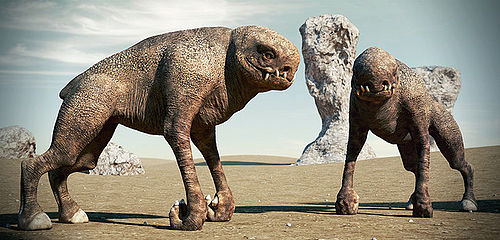
\includegraphics[scale=1.25]{sculpted_creatures.jpg}
  \caption{Цифровая скульптура инопланетных существ}
  \label{figure:domain:sculpting}
\end{figure}

\end{enumerate}

% References
% "3D Scanning Advancements in Medical Science". Konica Minolta. Retrieved 24 October 2011.
% Jon Radoff, Anatomy of an MMORPG Archived 2009-12-13 at the Wayback Machine., August 22, 2008
% "Lands' End First With New 'My Virtual Model' Technology: Takes Guesswork Out of Web Shopping for Clothes That Fit".
% PRNewswire. Lands' End. February 12, 2004. Retrieved 2013-11-24.
% "All About Virtual Fashion and the Creation of 3D Clothing". CGElves. Retrieved 25 December 2015.
% "3D Clothes made for The Hobbit using Marvelous Designer". 3DArtist. Retrieved 9 May 2013.
% "What is 3D Printing? The definitive guide". 3D Hubs. Retrieved 2017-11-18.
% "3D Printing Toys". Business Insider. Retrieved 25 January 2015.
% "Printout3D—Wolfram Language Documentation". reference.wolfram.com. Retrieved 2016-08-06.
% "New Trends in 3D Printing – Customized Medical Devices". Envisiontec. Retrieved 25 January 2015.
 %Sikos, L. F. (2016). Rich Semantics for Interactive 3D Models of Cultural Artifacts. Communications in Computer and
 %Information Science. 672. Springer International Publishing. pp. 169–180. doi:10.1007/978-3-319-49157-8_14.
 %Yu, D.; Hunter, J. (2014). "X3D Fragment Identifiers—Extending the Open Annotation Model to Support Semantic Annotation
 %of 3D Cultural Heritage Objects over the Web". International Journal of Heritage in the Digital Era. 3 (3): 579–596.
 %doi:10.1260/2047-4970.3.3.579.